\documentclass[11pt]{article}

% basic packages
\usepackage[margin=1in]{geometry}
\usepackage[pdftex]{graphicx}
\usepackage{amsmath,amssymb,amsthm}
\usepackage{notes}
\usepackage{lipsum}

% page formatting
\usepackage{fancyhdr}
\pagestyle{fancy}
\usepackage{hyperref}
\usepackage{tcolorbox}

\renewcommand{\sectionmark}[1]{\markright{\textsf{\arabic{section}. #1}}}
\renewcommand{\subsectionmark}[1]{}
\lhead{\textbf{\thepage} \ \ \nouppercase{\rightmark}}
\chead{}
\rhead{}
\lfoot{}
\cfoot{}
\rfoot{}
\setlength{\headheight}{14pt}

\linespread{1.03} % give a little extra room
\setlength{\parindent}{0.2in} % reduce paragraph indent a bit
\setcounter{secnumdepth}{2} % no numbered subsubsections
\setcounter{tocdepth}{2} % no subsubsections in ToC

\begin{document}

% make title page
\thispagestyle{empty}
\bigskip \
\vspace{0.1cm}

\begin{center}
{\fontsize{22}{22} \selectfont Compiled Notes from}
\vskip 16pt
{\fontsize{36}{36} \selectfont \bf \sffamily CERN OSAP}
\vskip 24pt
{\fontsize{18}{18} \selectfont \rmfamily Prannaya Gupta} 
\vskip 6pt
{\fontsize{14}{14} \selectfont \ttfamily prannayagupta@gmail.com} 
\vskip 24pt
\end{center}

{\parindent0pt \baselineskip=15.5pt This is gonna be fun.}

% make table of contents
\newpage
\microtoc
\newpage

% main content
\section{Fundamental Physics with Accelerators \\
\large{\it{by Albert De Roeck}}}

Physics, and Science as a whole, is largely predicated on answering major philosophical questions, which are considered \textbf{fundamental questions}. These questions are majorly supposed to clarify the extent of our understanding of the universe, such as the following:
\begin{itemize}
    \item What is the world made of?
    \item What holds the world together?
    \item Where did we come from?
\end{itemize}

This is summarised as follows:

\begin{figure}[h]
    \centering
    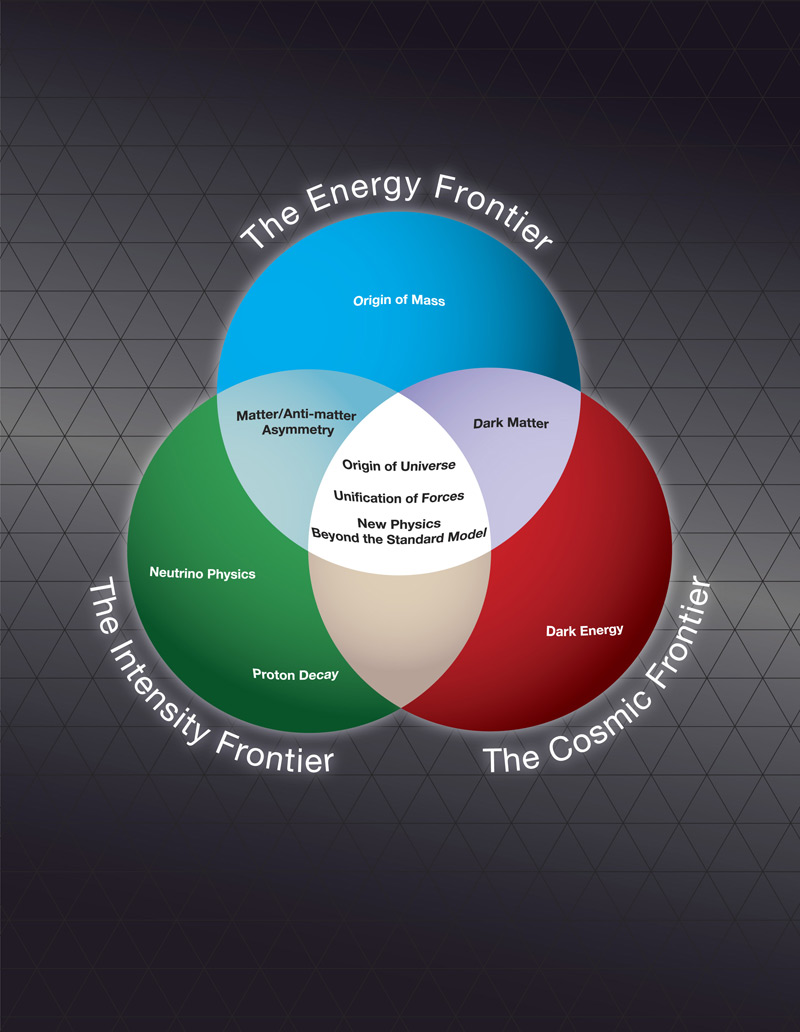
\includegraphics[width=0.5\textwidth]{images/three-frontiers.jpg}
    \caption{The Three Frontiers is Physics}
    \label{fig:frontiers}
\end{figure}


\end{document}